\documentclass[a4paper,12pt]{article}
\author{}

\usepackage{mathtools}
\usepackage{cancel}
\usepackage[utf8x]{inputenc}
\usepackage{blkarray}
\usepackage{amsmath}
\usepackage{amsthm}
\usepackage{commath}
\usepackage[english]{cleveref}
\usepackage[english]{babel}
\usepackage{graphicx}
\usepackage{booktabs}
\usepackage{arydshln}
\usepackage[toc,page]{appendix}
%
\usepackage[group-digits = false]{siunitx}
\usepackage[T1]{fontenc}
\DeclareSIUnit[number-unit-product = {}]{\inchQ}{\textquotedbl}
%
\usepackage{fixmath}
\usepackage{float}
\usepackage{enumerate}
\usepackage{subcaption}
\usepackage{caption}

%\usepackage{booktabs}
%, style=alphabetic, %style=reading

\graphicspath{ {figures/} }

%\renewcommand{\vec}[1]{\underline{#1}}
%\renewcommand{\vec}[1]{\mathbf{#1}}
\renewcommand{\vec}[1]{\boldsymbol{#1}}
\newcommand{\matr}[1]{\boldsymbol{#1}}
\newcommand{\unitvec}[1]{\hat{\mathbf{#1}}}
\newtheorem*{dualityprinciple}{Duality Principle}

\begin{document}

\tableofcontents
\newpage
\section*{Introduction}
In Robotics one of the most interesting task is the manipulation of objects. In general
it can be distinguished between the task of restraining objects, called grasping,
and the task of manipulating objects with fingers called dexterous manipulation.
\par
%% Among the hand-like end-effectors equipped with fingers proposed in the literature
%% there is the Pisa/IIT SoftHand.
The Pisa/IIT Hand \cite{Catalano2014} is one example of end-effector recently coined as soft hands.
It is simple because driven by one motor only
but at the same time robust because it adapts itself to the shape of grasped objects.
\par
Altough very versatile the simplicity of the hand make the grasp of thin objects,
such as a credit card or a sheet of paper, a very hard task
because such objects do not provide enough contact constraints to shape the hand during the grasp execution. %% on the hand
%% for the grasp to take place.
\par
Recent studies \cite{Bonilla2015} propose to face this problem taking into account
and exploiting hand-environment interaction. For example an object placed on a table
can be dragged until it reacheas the edge of the table and sticks out of it.
Then a standard grasp can be performed as usual. However in order to make
this solution workable the problem of making the dragging phase \emph{safe} must be faced.
Using a \emph{pure position} control strategy the \emph{uncontrolled} contact forces and torques
arising between the hand and the object and between the object and the surface of the table
could damage the object or the hand itself.
\par
In this project a \emph{hybrid force position} controller was implemented and tested on the
scenario described above to show that a force feedback solution allows to accomplish the task safely.
\par
The implementation was done using the ROS Control architecture and the robot used
in the experimental setup was a KUKA LWR $4+$ manipulator.

\subsection*{Contents description}
In section one the task of interest is briefly recalled
and a number of reference frames are introduced. They will be useful
to identify the quantities involved in the design of the controllers.
\par
In section two the main controller which realizes the hybrid
force position strategy is designed by choosing appropriate ``robot impedances''
for each degree of freedom within the so-called \emph{Hybrid Impedance (HIC)} framework
proposed by Spong in the 80s.
\par
In section three the synthesis of an inner loop inverse dynamics
controller, which is required by the HIC, is discussed. Also the issues of
controlling a kinematically redundant robot, like the LWR $4$+ in the case
of the task described, in the operational space
are discussed and solved using a \emph{dynamically consistent
generalized inverse} of the Jacobian from Khatib.
\par
In section four the Newton-Euler equations are written for
a rigid body attached to a common force/torque sensor in order to understand
how to obtain the measure of the contact forces and torques from the raw
signal of the sensor. This measure is required as a feedback signal within the
HIC framework. Also a simple least squares like approach is proposed
to estimate the mass of the rigid body, its center of mass and some software
induced offset introduced by the sensor itself.
\par
In section five a joint inverse dynamics controller with inverse
kinematics is developed. This controller is used to move the hand near
the object of interest when the starting configuration of the hand
is too far from the object and the HIC controller can not be used due
to the singularities in the attitude parametrization used in HIC
and due to the joints limits that are not handled in HIC.

\par
In the ending section the experimental setup is presented together with
the results of several experiments.
\newpage

%metti esperimento
\section{Description of the task}\label{sec:task_description}
This section serves as a preliminary one for the rest of the report. The main task
of interest is briefly recalled and several frames of reference are introduced within
the typical setup in which the task is performed. These frames of reference, along
with some notations and conventions, will be useful to easily identify the quantities
that belong to the state of the controllers developed in the next sections of this report.

\subsection{Typical set-up}
The typical setup, as shown in figure \ref{fig:frames}, consists of a $7$-joints KUKA LWR $4$+
anthropomorphic manipulator equipped with an hand-like end-effector, a table and an object that the hand is not
able to grasp using its primitives.
\begin{figure}[h]
  \centering
  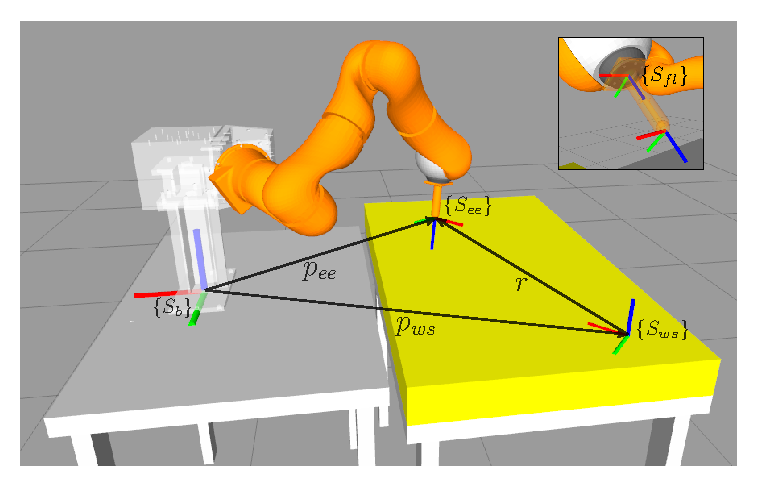
\includegraphics[scale=0.9]{frames.pdf}
  \caption{Typical set-up with reference frames \label{fig:frames}}
\end{figure}
Then the task to be performed consists in dragging the object on the table, hence exploiting
the environonmental constraints offered by the surface of the table, until the object sticks
out of the border of the table and a standard grasp is feasible. Also the dragging phase should
be accomplished without damaging the object or the hand because of too high contact forces between
the object and the surface of the table or between the object and the hand.
For this reason the manipulator is equipped with a force/torque sensor which is rigidely attached
to the last link of the robot and measures forces and torques exchanged at the wrist of the robot.
The hand is connected to the sensor using a mounting plate and a clamp.

\subsection{Division of the task in phases}\label{sec:task_division}
The dragging phase described above can be considered as the \emph{final} part of a more
complex task which should be divided, at least, in three parts:
\begin{itemize}
\item[-] approaching phase in which the robot moves the hand near the object of interest;
\item[-] contact phase in which the contact between the hand and the object takes place;
\item[-] dragging phase.
\end{itemize}

In the rest of the this report more attention is given to the dragging phase since it is the phase
where the hybrid force position strategy is used. As regards the contact phase the experimental results,
presented in the last section, show that it can be achieved using the same controller used in the dragging
phase. The approaching phase is also described in a separate section.

\subsection{Frames of reference}\label{sec:frames}
In order to develop a control system that is able to regulate the position of the object
and the force exerted on it, i.e. an hybrid force position control system, while the hand
is dragging the object on the table
a natural choice for a basis in which express the commanded positions and forces is that of
an inertial reference frame with the origin $W$ on a point of the table and the $x$ and $y$ axes parallel to the surface
of the table
\[
\{S_{ws}\} = \{W; x_{ws}, y_{ws}, z_{ws} \}
\]
where \emph{ws} stands for ``workspace'' since the table represents the intended workspace
for the robot. This choice allows to specify the commanded position as 2-dimensional vector
with components along the directions $\hat{\vec{i}}_{ws}$ and $\hat{\vec{j}}_{ws}$ and the
commanded force as a positive scalar along the direction $-\hat{\vec{k}}_{ws}$.
A quantity related to this reference frame is the vector $\vec{r}$ going from the origin $W$
to the center of the palm of the hand.
\par
A second reference frame to be introduced is an inertial frame fixed to the main base of the robot
\[
\{S_b\} = \{B; x_b, y_b, z_b \}
\]
Similarly to $\vec{r}$ the vector $\vec{p}_{ee}$ goes from $B$ to the center of the palm of the hand.
It should be noted that frames $\{S_{ws}\}$ and $\{S_b\}$ have no relative orientation and that
the vector $\vec{p}_{ws}$ going from $B$ to $W$ is constant. As a consequence the vector $\vec{r}(t)$
can be express as
\[
\vec{r}(t) = \vec{p}_{ee}(t) - \vec{p}_{ws}
\]
where $\vec{p}_{ws}$ is known and $\vec{p}_{ee}(t)$ is given by forward kinematics
numerical routines such as those offered by the library KDL used in this project.
The frame $\{S_b\}$ is also the frame in which the library KDL expresses quantities
like the vector $\vec{p}_{ee}$, the Jacobians and their derivatives.
\par
Other reference of frames of interest are those fixed to the end-effector
\[
\begin{split}
  &\{S_{fl}\} = \{F; x_{fl}, y_{fl}, z_{fl} \}\\
  &\{S_{ee}\} = \{E; x_{ee}, y_{ee}, z_{ee} \}
\end{split}
\]
where $F$ corresponds to the center of the wrist of the robot and $E$ is in the center
of the palm of the hand. These frames, that have no relative orientation,  are of interest
mainly because the signal produced by the force/torque sensor are expressed in these frames.

\subsection{Notation and convention}
In the rest of this report the following notation will be used to express any quantity $X$ encountered:
\[
\prescript{b}{}{X}_p
\]
where $b$ specify the reference frame $\{S_b\}$ in which $X$ is expressed and, whenever
$X$ is a wrench or a Jacobian $J$ such that $X\vec{\dot{q}}$ is a twist, $p$ specify the
reference point of that wrench or that twist. In case $X$ is an analytical Jacobian or $X$ is a vector
containing \emph{also} angular displacement or angular rates it should be clear that the specification
of a basis has no meaning and it applies only to a part of the vector.
\par
This notation is very general and sometimes the prescript $b$ and/or the subscript $p$ will
be missing when they are clear from the context.

\newpage


\section{Hybrid force position controller}
In this section the hybrid force position controller is presented.
With reference to the quantities introduced in the section \ref{sec:frames}
this controller should allow to regulate the position and the attitude of the hand
with respect to the frame $\{S_{ws}\}$ and at the same time the contact force between
the hand and the object expressed along the $z$ axis of the same frame.

\subsection{Desired dynamics of the error}\label{sec:desired_dyn}
In order to express the desired dynamics of the controlled system
more precisely the following error quantities are introduced
\[
e_x(t) =   \prescript{ws}{} r_{x,des}(t) - \prescript{ws}{} r_{x}(t)
\]
\[
e_y(t) =   \prescript{ws}{} r_{y,des}(t) - \prescript{ws}{} r_{y}(t)
\]
\[
\vec{e}_{\Phi}(t) = \vec{\Phi}_{des}(t) - \vec{\Phi}(t)
\]
where $\vec{r}$ is the vector from the origin $W$ of the frame $\{S_{ws}\}$ to the
center of the palm of the hand (see section \ref{sec:frames}) and $\vec{\Phi}$ is
a vector containing three angles that represent the orientation of the hand with respect
to the frame $\{S_{ws}\}$.
Also an error $e_z$ is defined as
\[
e_{z}(t) = \prescript{ws}{} F_{z,des}(t) - \prescript{ws}{} F_{z}(t)
\]
where $\prescript{ws}{} F_{z}$ is the force exerted by the hand on the object expressed
along the $\hat{\vec{k}}_{ws}$ direction.
\par
Using these definitions the desired dynamics of the error is expressed as
\[
\ddot{e}_{x} + B_x \dot{e}_x + K_x e_x = \vec{0} %\prescript{ws}{}{F}_x\\
\]
\[
\ddot{e}_{y} + B_y \dot{e}_y + K_y e_y = \vec{0} %\prescript{ws}{}{F}_y\\
\]
\[
\ddot{\vec{e}}_{\Phi} + B_{\Phi} \dot{\vec{e}}_{\Phi} + K_{\Phi} \vec{e}_{\Phi} = \vec{0} %\prescript{ws}{}{M}
\]
\[
e_z \xrightarrow[t \to \infty]{} 0
\]
The first two equations express the fact that the end-effector should rigidely follow
a given trajectory on a plane parallel to the surface of the table in a second order damped
fashion ($K$ and $B$ represent the proportional and damping terms).
The same reasoning applies for the attitude (third equation).
Finally the fourth equation only requires that the steady state force error should be zero.

\subsection{Definition of a state vector}
In order to develop a controller with the features described above
and \emph{operational}  state space vector is defined as
\begin{equation}
  \label{eq:state_space}
  \prescript{ws}{}{\vec{x}} = 
  \begin{bmatrix}
    \prescript{ws}{} r_x & \prescript{ws}{} r_y & \prescript{ws}{}r_z & \psi & \theta & \phi
  \end{bmatrix}^T
\end{equation}
where the angles $\psi$, $\theta$ and $\phi$ are the Euler ZYZ parametrization of the rotation matrix
$\prescript{ws}{}{R}_{ee}$ between the frames $\{S_{ws}\}$ and $\{S_{ee}\}$
\[
\prescript{ws}{}{R}_{ee} = R_{ZYZ}(\psi, \theta, \phi) = R_{ZYZ}(\vec{\Phi})
\]
Even though the force $\prescript{ws}{} F_z$ does not appear directly in the state vector
by making the hypothesis that the second derivative of the state can be commanded arbitrarily
\begin{equation}\label{eq:ddx_acmd}
\prescript{ws}{}{\ddot{\vec{x}}} = \vec{a}_{cmd}
\end{equation}
it will be shown that force can be regulated by an appropriate choice of term $\vec{a}_{cmd}$.
The hypothesis made above is a strong one and will be relaxed in the section \ref{sec:invdyn}
where an inverse dynamics inner loop controller will be developed for the manipulator.
This kind of controller allows to transform the non-linear dynamics of the manipulator in a
double integrator system of the form (\ref{eq:ddx_acmd}).

\subsection{Hybrid Impedance control strategy}
Among the various works on force control strategies available in the robot control
literature the strategy called \emph{Hybrid Impedance Control} proposed by Anderson and Spong
\cite{Anderson1988} was chosen due to its generality.
\par
The Hybrid impedance controller (HIC) combines the hybrid force/position control
with an impedance based control approach.
\par
Hybrid force/position control was first proposed by Raibert and Craig \cite{Raibert1981} and
allows to assign different control strategies to each 
Cartesian degree of freedom using some selection matrices. However it neglects the
importance of the manipulator impedance as seen by the environment during the interaction with it.
\par
The concept of impedance proposed by Anderson an Spong is more general with respect to the common
impedance approach in which a PD position controller is implemented with position and velocity
feedback gains adjusted to obtain different apparent impedances. First of all the
impedance control is performed in operational space so that an apparent impedance can be imposed
regardless of the configuration of the manipulator. Moreover the concept of impedance proposed
allows to synthesize \emph{direct force} control schemes by matching a given ``environment impedance''
with the appropriate ``manipulator impedance''.
\par
In the following the HIC approach is explained in more details
and a control law $\vec{a}_{cmd}$ is designed in order to fulfill
the control objectives described in \ref{sec:desired_dyn}.

\subsection{Frequency domain impedances}
A central concept in the HIC framework is that of frequency domain impedances.
A complex number of the form 
\begin{equation}
  \label{eq:impedance}
  Z(\omega)=R(\omega)+jX(\omega)
\end{equation}
with real part $R(\omega)$ and imaginary part $X(\omega)$, which resembles the Laplace
transform between a generalized effort and flow for a linear system, is used to model
both the environment and the manipulator \emph{for each} degree of freedom
avilable. It should be noted that in this framework
the environment is defined to be any element connected to or
contacting the robot anywhere past the wrist force sensor.
\begin{figure}[h]
  \centering
  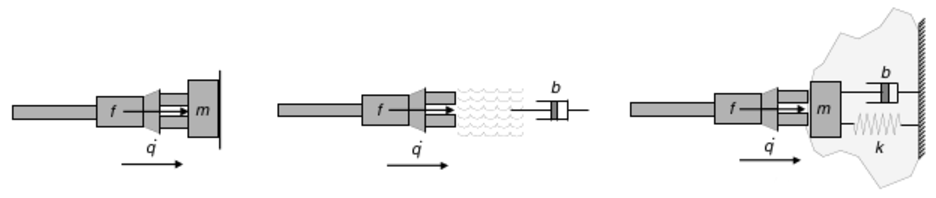
\includegraphics[scale=0.9]{type_of_impedances.pdf}
  \caption{Type of impedances. \label{fig:type_of_impedances}}
\end{figure}
\par
Impedances can be classified depending upon their \emph{low-frequency} behavior.
As $\omega$ approaches zero, one of three things can happen to 
the magnitude of the environment's and robot's impedance. It can 
approach infinity, it can approach a non-zero finite number or it can approach zero.
The following classification is now introduced:
\begin{itemize}
\item A system with impedance given by  (\ref{eq:impedance}) is \emph{inertial} IFF $\lim_{\omega \to 0}|Z(\omega)| = 0$ (Fig. \ref{fig:type_of_impedances}.a)
\item A system with impedance given by  (\ref{eq:impedance}) is \emph{resistive} IFF $\lim_{\omega \to 0}|Z(\omega)| = c$ where $0<c<\infty$ (Fig. \ref{fig:type_of_impedances}.b)
\item A system with impedance given by  (\ref{eq:impedance}) is \emph{capacitive} IFF $\lim_{\omega \to 0}|Z(\omega)| = \infty$ (Fig. \ref{fig:type_of_impedances}.c)
\end{itemize}

Capacitive, inertial and resistive systems are usually described in terms of 
Norton and Thèvenin equivalents. A capacitive system is 
represented by an impedance in parallel with a flow source (Norton).
An inertial system is represented by impedance in series with an 
effort source (Thévenin). Finally a resistive system 
can be either represented by a Thèvenin or Norton equivalent.

\subsection{The duality principle}
Once the environment has been properly modelled, the 
desired manipulator response may be determined. A fundamental goal for 
designing a controller is zero steady-state error to a step 
input. This will be obtained if the following duality principle is applied.
\begin{dualityprinciple}
  The manipulator should be controlled to respond as the dual of the environment.
\end{dualityprinciple}
This principle is most easily described in terms of Norton and Thèvenin equivalents.
An inertial environment, represented using a Thèvenin equivalent (Fig. \ref{fig:position_control_model}), is controlled by a manipulator represented by a non-inertial impedance.
\begin{figure}[h]
  \centering
  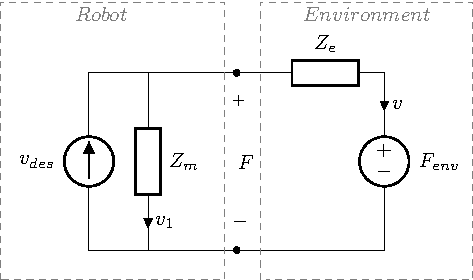
\includegraphics[scale=0.9]{position_control_model.pdf}
  \caption{Inertial environment. \label{fig:position_control_model}}
\end{figure}
Using the superposition principle the current (velocity) $v$ can be evaluated
\begin{equation}
  \label{eq:position_control_circuit}
  v = \frac{Z_m(s)}{Z_m(s) + Z_e(s)}v_{des} - 		\frac{F_{env}}{Z_e + Z_m}
\end{equation}
and the steady state error, assuming no environmental input ($F_{env} \equiv 0$) is equal to 
\[
e_{ss} \Big|_{F_{env}(t) \equiv 0} = \lim_{s \to 0}(v - v_{des}) = \frac{-Z_e(0)}{Z_m(0) + Z_e(0)}
\]
Since the the environment is inertial by hypothesis ($|Z_e(0)| = 0$) a choice of a non-inertial manipulator impedance ($Z_m(0) \neq 0$)
assures that
\[
e_{ss} \Big|_{F_{env}(t) \equiv 0} = 0
\]
So inertial environments are position controlled with a non-inertial manipulator impedances.
\par
A capacitive environment, represented using a Norton equivalent (Fig. \ref{fig:force_control_model}), 
is controlled by a manipulator represented by a 
non-capacitive impedance.
\begin{figure}[h]
  \centering
  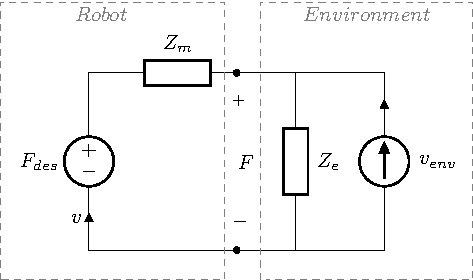
\includegraphics[scale=0.9]{force_control_model.pdf}
  \caption{Capacitive environment. \label{fig:force_control_model}}
\end{figure}
Using the superposition principle the voltage (force or torque) $F$ can be evaluated
\begin{equation}
  \label{eq:force_control_circuit}
  F = \frac{Z_e(s)}{Z_m(s) + Z_e(s)}F_{des} + \frac{Z_e Z_m}{Z_m + Z_e} V_{env}
\end{equation}

and the steady state error, assuming no environmental input ($v_{env} \equiv 0$) is equal to 
\[
e_{ss} \Big|_{v_{env}(t) \equiv 0} = \lim_{s \to 0}(F - F_{des}) = \frac{-Z_m(0)}{Z_m(0) + Z_e(0)}
\]
Since the environment is capacitive by hypothesis ($Z_e(0) \rightarrow \infty$) a choice of a
non-capacitive manipulator impedance ($Z_m(0) < \infty$) assures that
\[
e_{ss} \Big|_{v_{env}(t) \equiv 0} = 0
\]
So capacitive environments are force controlled with non-capacitive manipulator impedances.

\subsubsection{Position control}
The transfer function for the position-controlled circuit given in the Equation
(\ref{eq:position_control_circuit}) can be realized as a control scheme where the contact force is fed back.
Figure \ref{fig:position_control_feedback} shows a block diagram of the position-control implementation
\begin{figure}[h]
  \centering
  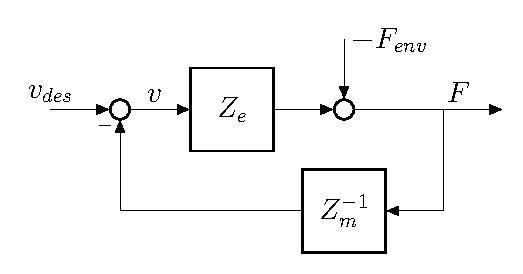
\includegraphics[scale=0.9]{position_control_feedback.pdf}
  \caption{Position control feedback. \label{fig:position_control_feedback}}
\end{figure}.
The commanded acceleration can be obtained from the velocity $v$ as
\[
a = \frac{\mathrm{d}}{\mathrm{d}t} \left(v_{des} - \frac{F}{Z_m}\right)
\]
In practice, the control $a$ can be obtained without use of differentiators
using only the measured force $F$, the end-effector position $x$ and velocity $\dot{x}$.
This is possible only if the manipulator impedance is expressed in a special form
\[
Z_m = Ms + \tilde{Z}_{m}
\]
where $M$ is a tuning parameter.
\par
Finally the position control law evaluates to
\begin{equation}
  \label{eq:position_law}
  a = \dot{v}_{des} + (v_{des} - v)\frac{\tilde{Z}_m}{M} - \frac{F}{M}
\end{equation}

\subsubsection{Force control}
The transfer function for the force-controlled circuit given in Equation (\ref{eq:force_control_circuit})
can also be realized as a force feedback scheme.
Figure \ref{fig:force_control_feedback} shows a block diagram of the force-control implementation.
\begin{figure}[h]
  \centering
  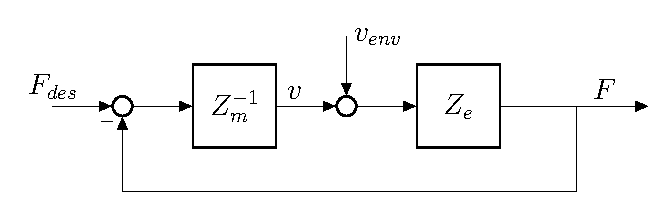
\includegraphics[scale=0.9]{force_control_feedback.pdf}
  \caption{Force control feedback. \label{fig:force_control_feedback}}
\end{figure}
Again the commanded acceleration can be obtained from the velocity $v$ as
\[
a = \frac{\mathrm{d}}{\mathrm{d}t} \left(\frac{F - F_{des}}{Z_m} \right)
\]
As done before for the position-controlled DoF $a$ can be obtained without differentiators if
the manipulator impedance assume the form
\[
Z_m = Ms + \tilde{Z}_{m}
\]
The force control law can then be written as
\begin{equation}
  \label{eq:force_law}
  a = \frac{1}{M} (F - F_{des}) - \frac{1}{M}( \tilde{Z}_m v)
\end{equation}

\subsection{Design of the control law}
In order to fulfill the control objectives described in \ref{sec:desired_dyn}
the manipulator impedances were chosen as follow.
\par
For the position and attitude-controlled DoFs they are
\[
\begin{split}
  &Z_{m,p} = M_p s + \tilde{Z}_{m,p} = M_p s + B_p + \frac{K_p}{s}\\
  &Z_{m,a} = M_a s + \tilde{Z}_{m,a} = M_a s + B_a + \frac{K_a}{s}
\end{split}
\]
which result in the following acceleration commands
\[
\begin{split}
  &a_{p} = a_{des,p} + \frac{B_p}{M_p} (v_{des,p} - v_p) + \frac{K_p}{M_p} (x_{des,p} - x_p) - \frac{F_p}{M_p}\\
  &a_a = a_{des,a} + \frac{B_a}{M_a} (v_{des,a} - v_a) + \frac{K_a}{M_a} (x_{des,a} - x_a) - \frac{F_a}{M_a}
\end{split}
\]
For the force-controlled DoF the impdance is given by
\[
Z_{m,f} = M_f s + \tilde{Z}_{m,f} = M_f s + B_f
\]
which results in the control law
\[  
a_{f} = M_f^{-1}((f_{des} - f) - B_f v_z)
\]
In principle a position control law and a force control law could be assigned for each DoF. Since this
behavior is not possible physically a selection matrix $S$ is used to separate the force-controlled and position-controlled reciprocal subspaces
\[
\vec{a} = S 
\begin{bmatrix}
  \vec{a}_p \\
  \vec{a}_a
\end{bmatrix} + (I - S) \vec{a}_f
\]
where the vector $\vec{a}_p$ and $\vec{a}_a$ are the position and attitude control laws
\[
\begin{split}
  &\vec{a}_p = 
  \begin{bmatrix}
    a_{p,x} & a_{p,y} & a_{p,z}
  \end{bmatrix}^T\\
  &\vec{a}_a = 
  \begin{bmatrix}
    a_{a, \psi} & a_{a, \theta} & a_{a, \phi}
  \end{bmatrix}^T
\end{split}
\]
the vector $\vec{a}_f$ is the force/torque control law
\[
\vec{a}_f = 
\begin{bmatrix}
  a_{f,x} & a_{f,y} & a_{f,z} & a_{f, \psi} & a_{f, \theta} & a_{f, \phi}
\end{bmatrix}^T
\]
and $S$ is the selection matrix that for the set-up described in section \ref{sec:task_description} assumes the form
\[
S =
\begin {bmatrix}
  1 & 0 & 0 & 0 & 0 & 0\\
  0 & 1 & 0 & 0 & 0 & 0\\
  0 & 0 & 0 & 0 & 0 & 0\\
  0 & 0 & 0 & 1 & 0 & 0\\
  0 & 0 & 0 & 0 & 1 & 0\\
  0 & 0 & 0 & 0 & 0 & 1\\
\end {bmatrix}
\]
The resulting control laws is
\begin{equation}\label{eq:final_a_cmd}
\begin{cases}
\prescript{ws}{}{a}_1 = a_x = \ddot{r}_{x,des} + B_x (\dot{r}_{x,des} - \dot{r}_x) + K_x (r_{x,des} - r_x) - F_x \\
\prescript{ws}{}{a}_2 = a_y = \ddot{r}_{y,des} + B_y (\dot{r}_{y,des} - \dot{r}_y) + K_y (r_{y,des} - r_y) - F_y \\
\prescript{ws}{}{a}_3 = a_z = - B_f \dot{r}_z + K_f(F_{z,des} - F_z) \\
\prescript{ws}{}{a}_4 = a_{\psi} = \ddot{\psi}_{des} + B_{\psi} (\dot{\psi}_{des} - \dot{\psi}) + K_{\psi} (\psi_{des} - \psi) \\
\prescript{ws}{}{a}_5 = a_{\theta} = \ddot{\theta}_{des} + B_{\theta} (\dot{\theta}_{des} - \dot{\theta}) + K_{\theta} (\theta_{des} - \theta) \\
\prescript{ws}{}{a}_6 = a_{\phi} = \ddot{\phi}_{des} + B_{\phi} (\dot{\phi}_{des} - \dot{\phi}) + K_{\phi} (\phi_{des} - \phi)
\end{cases}
\end{equation}
where the ratios of the form $\frac{K}{M}$ or $\frac{B}{M}$ are substituted with $K$ and $B$ respectively.
\par
The desired trajctories for the position and attitude-controlled DoFs were chosen as  $5^\text{th}$ order polynomials of the form
\[
s(t) = a_5 t^5 + a_4 t^4 + a_3 t^3 + a_2 t^2 +a_1 t + a_0
\]
with boundary conditions
\[
\begin{split}
  &s(0) = s_0 \quad \dot{s}(0) = 0 \quad \ddot{s}(0) = 0\\
  &s(t_f) = s_f \quad \dot{s}(t_f) = 0 \quad \ddot{s}(t_f) = 0
\end{split}
\]
while the reference force trajectory was chosen as a $3^\text{th}$ order polynomial
\[
s(t) = a_3 t^3 + a_2 t^2 +a_1 t + a_0
\] 
with boundary conditions
\[
\begin{split}
  &s(0) = s_0 \quad \dot{s}(0) = 0\\
  &s(t_f) = s_f \quad \dot{s}(t_f) = 0
\end{split}
\]
\newpage

\section{Inverse Dynamics Inner Loop}\label{sec:invdyn}
In the previous section the hybrid force position control scheme was described
with the assumption that an inverse dynamics inner loop was available. In this
section the inverse dynamics controller is described and the issue of controlling
a kinematically redudant manipulator is discussed.

\subsection{Design of the inverse dynamics controller}
The development of the controller starts from the dynamic model of the 7-joint
manipulator
\begin{equation}\label{eq:joint_space_dyn}
  B(\vec{q}) \ddot{\vec{q}} + C(\vec{q}, \dot{\vec{q}}) \dot{\vec{q}} + \cancel{\vec{G}(\vec{q})} = \vec{\tau}
  -\prescript{b}{}{J}^{T}_{S} \prescript{b}{}{\vec{w}}_{S}
\end{equation}

where $\vec{w}_{S}$ is the wrench exerted by the hand on the environment
with reference point in the centre
of the sensor ($S$) and $J_{S}$ is the geometric Jacobian of the robot.
The gravity term is canceled because it is handled internally by the robot itself.
\par
The first step towards the exact dynamics inversion is to cancel the Coriolis term
$C \dot{\vec{q}}$ and the term containing the wrench $\vec{w}_{S}$ which is supposed to
be available as a feedback signal. The resulting control torque is then
\[
\vec{\tau} = C \dot{\vec{q}} + {}^{b}J^{T}_{S} ({}^b\vec{\gamma} + {}^b\vec{w}_{S})
\]
where an additional control wrench $\vec{\gamma}$ is introduced.
Substituing the control torque and solving for the joints accelerations $\vec{\ddot{q}}$
leads to
\begin{equation}\label{eq:qddot}
  \ddot{\vec{q}} = B^{-1} ({}^{b}J^{T}_{S}) {}^b\vec{\gamma}
\end{equation}
\par
The link between the joint space description and the operational space description
is given by the following formula
\begin{equation}
  \label{eq:ws_a}
  {}^{ws} \ddot{\vec{x}} = {}^{ws} J_{A,E} \ddot{\vec{q}} + {}^{ws} \dot{J_{A,E}} \dot{\vec{q}}
\end{equation}
where ${}^{ws} \vec{x}$ is the previously introduced (eq \ref{eq:state_space}) state in operational space expressed in workspace
frame and $J_{A,E}$ is the analytical Jacobian of the robot with reference point in the palm of the hand.
The analytical Jacobian, which takes into account the conversion between the angular velocity $\vec{\omega}$
and the vector of angular rates $\vec{\dot{\Phi}}$, can be written as
\[
\prescript{ws}{}{J}_{A,E} = 
\begin{bmatrix}
  I & 0 \\
  0 & T^{-1}(\vec{\Phi})
\end{bmatrix}
\prescript{ws}{}{J}_{E} \quad {}^{ws}\vec{\omega} = T(\vec{\Phi}) \vec{\dot{\Phi}}
\]
with $J_E$ the geometric Jacobian with reference point int the palm of the hand. It should be noted
that the inverse of the matrix $T$ exists if and only if the sine of the angle $\theta$ (part of the state
$\vec{x}$) is not zero. The derivative of the analytical Jacobian evaluates to
\[
\prescript{ws}{}{\dot{J}}_{A,E} = 
\begin{bmatrix}
  0 & 0 \\
  0 & -T^{-1} \dot{T} T^{-1}
\end{bmatrix}
\prescript{ws}{}{J}_{E} + 
\begin{bmatrix}
  I & 0 \\
  0 & T^{-1}
\end{bmatrix}
\prescript{ws}{}{\dot{J}}_{E}
\]
where the derivative of the Jacobian $\dot{J}_{E}$ can be evaluated numerically
using software libraries like KDL (Kinematics and Dynamics Library).
\par
By substituing equation (\ref{eq:qddot}) in equation (\ref{eq:ws_a}) one obtains
\[
\prescript{ws}{}{\ddot{\vec{x}}} = \underbrace{\prescript{ws}{}{J}_{A,E} B^{-1} ({}^b J_{S}^T)}_{\Lambda_A^{-1}} {}^b \vec{\gamma} + {}^{ws} \ddot{J_{A,E}} \dot{\vec{q}}
\]
where the kinetic psuedo-kinetic energy matrix $\Lambda_{A}$ was introduced. Multiplying both sides of the equation
by $\Lambda_{A}$ leads to
\[
\Lambda_A {}^{ws} \ddot{\vec{x}} =  {}^b \vec{\gamma} +  \Lambda_A  {}^{ws} \dot{J_{A,E}} \dot{\vec{q}}
\]
where the control wrench $\gamma$ can now be easily chosen as
\[\label{eq:gamma}
\vec{\gamma} = \Lambda_A \vec{a}_{cmd} - \Lambda_A {}^{ws} \dot{J_{A,E}} \dot{\vec{q}}
\]
resulting in
\[
\prescript{ws}{}{\ddot{\vec{x}}} = \vec{a}_{cmd}
\]
where $\vec{a}_{cmd}$ represents the outer control expressed in equation (\ref{eq:final_a_cmd}).
Taking into account the command wrench $\vec{\gamma}$ the final commanded torque is
\begin{equation}\label{eq:torque_wo_null}
  \vec{\tau} = C \dot{\vec{q}} + {}^{b}J^{T}_{S} ( B_A \vec{a} - B_A {}^{ws} \dot{J_{A,E}} \dot{\vec{q}} + {}^b\vec{w}_{S})
\end{equation}

\subsection{Control of redundant manipulators}
The control law presented in the previous subsection does not take into account
the fact that the controlled manipulator is kinematically redundant. In fact it has
7 joints while the commanded state in the operational space is 6-dimensional.
A consequence of this fact is that \cite{Khatib1987} the configuration of the robot, which describes the
end-effector position and orientation, does not constitute a generalized coordinate
system for the whole redundant manipulator and the dynamic behavior of the entire redundant
system cannot be represented by a dynamic model in coordinates only of the end-effector
configuration. Indeed it turns out that the command torques specified in equation (\ref{eq:torque_wo_null}),
altough they specify univocally the behavior of the end-effector, they are none other than one of the
possible torques producing a given operational command wrench $\vec{\gamma}$ on the end-effector, i.e,
the expression
\begin{equation}\label{eq:torques_gamma}
  \vec{\tau} = J^{T} \vec{\gamma}
\end{equation}
represents just one of these torques. Clearly different torques lead to completely different behaviors
of the additional degree of freedom of a kinematically redundant manipulator, some of which may be undesired
or even dangerous. For this reason a complete characterization of the torques producing a given command wrench
at the end-effector is necessary to avoid this issue.
\par
Independently of the specific choice for the operational space description of the robot
the second derivative with respect to time of the state can be written in the form
\begin{equation}\label{eq:xddot}
  \vec{\ddot{x}} = J(\vec{q}) \vec{\ddot{q}} + \vec{h}(\vec{q},\vec{\dot{q}})
\end{equation}
for some Jacobian matrix $J$ and some function of the joints state and velocity $\vec{h}$.
By combining equations (\ref{eq:joint_space_dyn}), in the case of zero contact forces,
(\ref{eq:torques_gamma}) and (\ref{eq:xddot}) the equations of motion of the end-effector
are obtained
\begin{equation}\label{eq:operational_space_dyn}
  \Lambda \vec{\ddot{x}} + \vec{\mu}(\vec{q}, \vec{\dot{q}}) + \vec{p} = \vec{\gamma}
\end{equation}
where
\[
\Lambda = (J B^{-1} J^{T})^{-1}
\]
\[
\vec{\mu} = \bar{J}^{T} C \vec{\dot{q}} - \Lambda \vec{h}
\]
\[
\vec{p} = \bar{J}^T \vec{G}
\]
are the already seen pseudo-kinetic energy matrix, the centrifugal and
Coriolis forces acting on the end-effector and the gravity force acting on the end-effector
respectively.
The matrix $\bar{J} = B^{-1} J^{T} \Lambda$ is a generalized inverse of the Jacobian matrix
which solves the problem of finding the joints velocities that produce a desired twist
while minimizing the manipulator's instantaneous kinetic energy.
\par
Interestingly equation (\ref{eq:operational_space_dyn}) can also be written in the form
\[
\bar{J}^{T} (B \vec{\ddot{q}} + C \vec{\dot{q}} + \vec{G}) = \vec{\gamma}
\]
Since the joint space dynamics term that is multiplied by $\bar{J}^{T}$ is equal to the
commanded torque $\vec{\tau}$ one finds that
\begin{equation}\label{eq:gamma_torques}
  \vec{\gamma} = \bar{J}^{T} \vec{\tau}
\end{equation}
which is an important result since it allows to design a command torque $\vec{\tau}$ of the form
\begin{equation}\label{eq:torque_w_null}
  \vec{\tau} = J^{T} \vec{\gamma} + (I_7 - J^{T}\bar{J}^{T}) \vec{\gamma}_{0}
\end{equation}
where the command wrench $\vec{\gamma}_{0}$ is projected in the null space of the
generalized inverse $\bar{J}^{T}$ hence, as results by direct substitution of equation
(\ref{eq:torque_w_null}) in equation (\ref{eq:gamma_torques}), it corresponds
to a \emph{null} operational wrench command. Clearly the term $\vec{\gamma}_{0}$ can
be used to avoid undesired motion of the additional degree of freedom of the manipulator
without interfering with the desired motion of the end-effector.
\par
It should be noted that the expression in equation (\ref{eq:torque_w_null}) is very general, i.e.,
every commanded torque $\vec{\tau}$ can always be expressed in that form.
Also due to its filtering capabilities the matrix $\bar{J}$ is called \emph{dynamically consistent generalized inverse} 
of $J$ in the sense that the projector in the null of $\bar{J}^T$ is able 
to filter out commanded wrenches in a way that is consistent with the dynamics of both the
whole manipulator and the end-effector.
\par
Taking into account the development presented in this section the commanded torques $\vec{\tau}$
in equation (\ref{eq:torque_wo_null}) are updated to
\begin{equation}\label{eq:torqu_w_null_1}
  \vec{\tau} = C \dot{\vec{q}} + {}^{b}J^{T}_{S} ( \Lambda_A \vec{a} - \Lambda_A {}^{ws} \dot{J_{A,E}} \dot{\vec{q}} + {}^b\vec{w}_{S}) +
  (I_7 - ({}^{b}J^{T}_{S}) ({}^{b} \bar{J}^{T}_{S})) \vec{\gamma}_{0}
\end{equation}
where
\[
\prescript{b}{}{\bar{J}}_{S} = B^{-1} ({}^{b} J^{T}_{S}) ({}^{b} \Lambda_{S})
\]
and
\[
\prescript{b}{}{\Lambda}_{S} = ({}^{b} J_{S} B^{-1} ({}^{b} J^{T}_{S}))^{-1}
\]

\subsubsection{Design of the null operational wrench command}
Design of the control law assigned to the term $\vec{\gamma}_{0}$ was
guided by the simulation of the task described in section \ref{sec:task_description}. Extensive simulations
revealed that the uncontrolled internal motions of the robot, while not affecting the desired
attitude of the hand, caused the $5$-th and $7$-th links to rotate cooperatively and reach
their limits soon. Another issue with internal motions is that they could cause, in some situations,
collisions between the $4$-th link and the table which is part of the workspace of the robot.
\par
In order to handle the issues described the control $\vec{\gamma}_0$ was choosen as
\[
\vec{\gamma}_{0} = J_{im} ^{T} (K_p (\vec{x}_{im,des} - \vec{x}_{im} ) - K_d \vec{\dot{x}}_{im})
\]
where \emph{im} stands for ``internal motion'', the state $\vec{x}_{im}$
\[
\vec{x}_{im} =
\begin{bmatrix}
  {}^{b} x_{l4} & {}^{b} y_{l4} & {}^{b} z_{l4} & \psi_{l5} & \theta_{l5} & \phi_{l5}
\end{bmatrix}^{T} =
\begin{bmatrix}
  \vec{p}^{T}_{l4} & \vec{\Phi}^{T}_{l5}
\end{bmatrix}^{T}
\]
describes the position, with respect to the base of the robot, of the $4$-th link
and the attitude of the $5$-th link using a ZYZ parametrization and the Jacobian
$J_{im}$ is such that
\[
\begin{bmatrix}
  \vec{\dot{p}}_{l4} \\
  \vec{\dot{\Phi}}_{l5} \\
\end{bmatrix} =
J_{im} \vec{\dot{q}}
\]
\par
The gains $K_p$ and $K_d$ and the desired state $\vec{x}_{im,des}$ were chosen as
\[
K_p = \text{diag}(0, 0, k_{p,z}^{im}, 0, 0, k_{p, att}^{im})
\quad
K_d = k_{d}^{im} I_{6}
\]
\[
\vec{p}_{l4} =
\begin{bmatrix}
  * & * & {}^{b} z_{ee} + off_z
\end{bmatrix}^{T}
\quad
\vec{\Phi}_{l5} =
\begin{bmatrix}
  * & * & 0\\
\end{bmatrix}^{T}
\]
where ${}^{b} z_{ee}$ is the altitude of the hand with respect to the base of the robot
and $k_{p,z}^{im}$, $k_{att}^{im}$ and $k_{d}^{in}$ are suitable gains.
Such a choice allows to fix the orientation of the $5$-th link to a value that is comfortable
during the execution of task described in the section \ref{sec:task_description} and to regulate the altitude between the $4$-th link and
the hand so as to avoid collisions between the elbow of the robot and the workspace.
\newpage

\section{Measure of the contact forces and torques}
In the previous sections the hybrid force-position control architecture was described
and the assumption was made that the wrench $\vec{F}_{ee, env}$ exerted by the end effector on the environment
was available as a feedback signal.
\par
In this section it is explained how such a wrench can be obtained starting from the \emph{raw} signal
coming from a common force/torque sensor and what are the main problems encountered in doing that.

\subsection{Newton-Euler equations}
In order to understand what are the actual quantities measured by a force/torque sensor it is useful
to describe, by means of the Newton-Euler approach, the motion of a rigid body, attached to the
sensor through a mounting plate, due to external forces and torques. The resulting equations are the following

\begin{equation}
  {}^S \vec{f}_{s} = -{}^S \vec{f}_{pl} -{}^S \vec{f}_{c} -m {}^S \vec{g} + m {}^S \vec{a}_{cm}
\end{equation}
\begin{equation}\label{eq:ne_torque_1}
  {}^S \vec{\tau}_{s} = -{}^S \vec{\tau}_{pl} -{}^S \vec{\tau}_{c} -{}^S \tilde{\vec{p}}_{c} {}^S \vec{f}_{c}
  +{}^S \tilde{\vec{g}} m{}^S\vec{c} - {}^S \tilde{\vec{a}}_{cm} m {}^S \vec{c} + {}^S I_{cm} {}^S\vec{\alpha} 
  +{}^S \tilde{\vec{\omega}} {}^S I_{cm} {}^S \vec{\omega}
\end{equation}
where $S$ denotes a reference frame fixed to the sensor body, as introduced in (cite prev sections),
$\vec{f}_{s}$ and $\vec{\tau}_{s}$ are the forces and torques exerted by the sensor on the rigid body,
$\vec{f}_{pl}$ and $\vec{\tau}_{pl}$ are due to the mounting plate,
$\vec{f}_{c}$ and $\vec{\tau}_{c}$ are the \emph{external} forces and torques exerted on the rigid body in the interaction
with the environment,
$\vec{c}$ is the vector from the wrist of the robot to the CoM of the rigid body,
$\vec{p}_{c}$ is the vector from wrist of the robot to the contact point with the environment,
$I_{cm}$ is the inertia matrix of the rigid body with respect to the CoM,
$\vec{g}$ is the gravity vector, $\vec{a}_{cm}$ is the linear acceleration of the CoM of the rigid body,
$\vec{\omega}$ is the angular velocity of the rigid body and
$\vec{\alpha}$ is the angular acceleration of the rigid body.
\par
It should be noted that the wrench $\vec{F}_{ee,env}$ with reference point in the contact point with the environment is given by
$\begin{bmatrix}
  & -\vec{f}_{c} ^T & - \vec{\tau}_{c} ^ T \\
\end{bmatrix}^T$
and that all the torques in equation (\ref{eq:ne_torque_1}) are expressed with the reference point in the wrist
of the robot where the sensor is mounted.
\par
Since in this project the force/torque sensor is primarily used to control the contact force when the end effector
is still or when it moves along straight lines the angular velocity and the angular acceleration of the end effector
attached to the sensor can be neglected leading to the equations
\begin{equation}\label{eq:ne_force_2}
   \vec{f}_{s} = - \vec{f}_{pl} - \vec{f}_{c} -m  \vec{g} + m  \vec{a}_{cm}
\end{equation}
\begin{equation}\label{eq:ne_torque_2}
   \vec{\tau}_{s} = - \vec{\tau}_{pl} - \vec{\tau}_{c} - \tilde{\vec{p}}_{c}  \vec{f}_{c}
  + \tilde{\vec{g}} m\vec{c} -  \tilde{\vec{a}}_{cm} m  \vec{c}
\end{equation}

\subsection{Software induced offset}
The hardware of the force/torque sensor is built in a such way that the forces and torques exchanged
with the rigid body attached to it are measured. With reference to the equations (\ref{eq:ne_force_2})
and (\ref{eq:ne_torque_2}) the signal produced by the sensor can be written as

\begin{equation*}
  \vec{f}_{m} = -\vec{f}_{s} + \vec{f}_{sw,off}
\end{equation*}
\begin{equation*}
  \vec{\tau}_{s} = -\vec{\tau}_{s} + \vec{\tau}_{sw,off}
\end{equation*}
where $\vec{f}_{sw, off}$ and $\vec{\tau}_{sw,off}$ represent the offset introduced by
the sensor when the user activates the \emph{calibration} of the sensor. This operation
is performed when the sensor is \emph{still} and not in contact with the environment
and the resulting offset is chosen such that $\vec{f}_{m,0} = \vec{\tau}_{m,0} = \vec{0}$
where the zero subscript represents the calibration condition. Simple substitutions show that
\begin{equation*}
\vec{f}_{sw,off} = \vec{f}_{s,0} = -\vec{\tau}_{pl} -m {}^S \vec{g}_{0}
\end{equation*}
\begin{equation*}
\vec{\tau}_{sw,off} = \vec{\tau}_{s,0} = -\vec{\tau}_{pl} + {}^S \tilde{\vec{g}_{0}} m\vec{c}
\end{equation*}
where $\vec{g}_{0}$ is the value assumed by the gravity expressed in the sensor frame $S$ at the
moment of the calibration.
\par
Taking into account the expressions of the offset the measured forces and torques in absence of angular
motions can be written as
\begin{equation}\label{eq:m_force_2}
  \vec{f}_{m} = \vec{f}_{c} +m \vec{g} -m {}^S \vec{g}_{0} - m  \vec{a}_{cm}
\end{equation}
\begin{equation}\label{eq:m_torque_2}
  \vec{\tau}_{m} = \vec{\tau}_{c} + \tilde{\vec{p}}_{c}  \vec{f}_{c}
  - \tilde{\vec{g}} m\vec{c} + {}^S \tilde{\vec{g}_{0}} m\vec{c} +  \tilde{\vec{a}}_{cm} m  \vec{c}
\end{equation}
As suggested by the previous formulas in order to obtain the part of the measure related to the contact
with the environment it is required to estimate the mass of the rigid body $m$, the position of the centre of
mass with respect to the wrist $\vec{c}$ and the offsets $-m {}^S \vec{g}_{0}$ and ${}^S \tilde{\vec{g}_{0}} m\vec{c}$.
The gravity ${}^S \vec{g}$ expressed in sensor frame can be obtained using the direct kinematics software facilities
developed for the project while the linear acceleration $\vec{a}_{cm}$ can be obtained using an appropriate
jacobian, its derivative and an estimate of the angular velocities and accelerations of the joints
of the robot.

\subsection{Estimation of parameters and offsets}
Since all the quantities to be estimated are revealed even when the sensor is still
it is possible to estimate them by acquiring a certain number of measures each when
the robot, hence the sensor, assumes a static pose. The estimation can be obtained
from the measures using a \emph{linear} least squares approach since there exist
a linear relationship between the measurements and the parameters

\begin{equation*}
  \begin{flalign*}
    \begin{bmatrix}
      \vec{f}_{m} \\
      \vec{\tau}_{m} \\
    \end{bmatrix} &=
    \begin{bmatrix}
      \vec{g} m + (-m {}^S \vec{g}_{0}) \\
      -\tilde{\vec{g}} m\vec{c} + ({}^S \tilde{\vec{g}_{0}} m\vec{c}) \\
    \end{bmatrix}\\
    & =
    \begin{bmatrix}
      \vec{g} & 0_{3 \times 3} & I_{3x3} & 0_{3x3} \\
      \vec{0} & -\tilde{\vec{g}} & 0_{3x3} & I_{3x3}
    \end{bmatrix}
    \begin{bmatrix}
      m \\
      m \vec{c} \\
      -m {}^S \vec{g}_{0} \\
      {}^S \tilde{\vec{g}_{0}} m\vec{c} \\
    \end{bmatrix}\\
    &=
    H({}^S \vec{g}) \vec{\theta}
  \end{flalign*}
\end{equation*}
where ${}^S \vec{g} = {}^S \vec{g(\vec{q})}$ depends on the configuration $\vec{q}$ of the robot.
\par
Given n configurations of the robot the estimate is given by
\begin{equation*}
  \begin{flalign*}
    \hat{\vec{\theta}} &=
    \begin{bmatrix}
      H(\vec{q}^{1})\\
      \vdots \\
      H(\vec{q}^{n})\\
    \end{bmatrix}^{+}
    \begin{bmatrix}
      \vec{f}_{m}^{1} \\
      \vec{\tau}_{m}^{1} \\
      \vdots \\
      \vec{f}_{m}^{n} \\
      \vec{\tau}_{m}^{n} \\
    \end{bmatrix}
    =
    H_n^{+}
    \begin{bmatrix}
      \vec{f}_{m}^{1} \\
      \vec{\tau}_{m}^{1} \\
      \vdots \\
      \vec{f}_{m}^{n} \\
      \vec{\tau}_{m}^{n} \\
    \end{bmatrix}\\
  \end{flalign*}
\end{equation*}
where it can be shown that for $n \ge 3$ the matrix $H_n$ is always full column rank
so that $H_n^{+} = H_n(H_n^{T} H_n)^{-1}$.
Once the estimate is computed contact forces and torques can be evaluted as
\begin{equation*}
  \hat{\vec{f}}_c = \vec{f}_m - \hat{\theta}_{1} \vec{g} - \hat{\vec{\theta}}_{5:7} + \hat{\theta}_{1} \hat{\vec{a}}_{cm}(\vec{q},\vec{\dot{q}},\vec{\ddot{q}})
\end{equation*}
\begin{equation*}
  \hat{\vec{\tau}}_c + \tilde{\vec{p}}_{c}  \hat{\vec{f}}_{c} = \vec{\tau}_m
    + \tilde{\vec{g}} \hat{\vec{\theta}}_{2:4} - \hat{\vec{\theta}}_{8:10} -  \tilde{\hat{\vec{a}}}_{cm}}(\vec{q},\vec{\dot{q}},\vec{\ddot{q}}) \hat{\vec{\theta}}_{2:4}
\end{equation*}
where $\hat{\vec{a}}_{cm}$ is an estimate of the linear acceleration of the centre of mass of the rigid body.

\section{Approaching phase controller}
As explained in the section \ref{sec:task_division} before the execution of the dragging phase
a preliminar approaching phase is required  to move the hand near the object of interest.
\par
In principle the HIC controller could also be used to perform this task but in practice
some issues due to the singularity introduced by the Euler ZYZ parametrization and due to the
joints limits make that controller useful during the dragging phase only where short movements are executed
and the attitude is carefully commanded to avoid the singularity issue.
So another controller was developed using a joint space approach so that large movements can be performed.

\subsection{Design of a joint space point to point controller}
The alternative controller was developed combining an inverse dynamics controller in joint
space with an inverse kinematics solver.
\par
By substituing a command torque of the form
\[
\vec{\tau} = C(\vec{q}, \dot{\vec{q}}) \dot{\vec{q}} + \vec{G}(\vec{q}) + B(\vec{q}) \vec{a}
\]
in the joint space dynamics of the manipulator
\[
  B(\vec{q})\ddot{\vec{q}} + C(\vec{q}, \dot{\vec{q}}) \dot{\vec{q}} + \vec{G}(\vec{q}) = \vec{\tau}
\]
the following results
\[
\ddot{\vec{q}} = \vec{a}_{p2p}
\]
where $\vec{a}_{p2p}$ is the new input vector.
\par
In order to move the hand from the previous configuration $\vec{q}_{prev}$
to a new one expressed as a position in cartesian coordinates $\vec{p}_{ee}$ and
an orientation $\prescript{b}{}{R}_{ee}$ a joint space trajectory was generated
\[
q_{des}^{i}(t) = a_0 + a_1 t + a_2 t^2 + a_3 t^3 + a_4 t^4 + a_5 t^5
\]
with boundary conditions
\[
\begin{split}
  &q_{des}^{i}(0) = q_{prev}^{i} \quad \dot{q}_{des}^{i}(0) = 0 \quad \ddot{q}_{des}^{i}(0) = 0\\
  &q_{des}^{i}(t_f) = q_{f}^{i} \quad \dot{q}_{des}^{i}(t_f) = 0 \quad \ddot{q}_{des}^{i}(t_f) = 0
\end{split}
\]
where $\vec{q}_{f}$ is given by an inverse kinematics solver
\[
\vec{q}_{f} = FK^{-1}(\vec{p}_{ee,des},\prescript{b}{}{R}_{ee,des})
\]
and is discarded whenever its components exceed the joints limits.
\par
In order to execute the trajectory an input vector of the form
\[
\vec{a}_{p2p} = \ddot{\vec{q}}_{des} + K_d(\dot{\vec{q}}_{des} - \dot{\vec{q}}) + K_p(\vec{q}_{des} - \vec{q})
\]
was used where $K_p$ and $K_d$ are positive definite matrices.
\newpage

\section{Experimental setup and results}
In this section the experimental setup is described and the 
results of three experiments are presented.
In the first one the robot is supposed to press an emergency button with variables
force references. In the second and in the third one the robot drags an object on a table 
while the contact force is regulated until 
it reaches the edge of the table and sticks out of it.

\subsection{Experimental setup}
The test-bed for this project is a Kuka LWR$4+$, a $7$-joints industrial manipulator, 
which is provided with an internal software layer called Fast Research Interface (FRI).
\begin{figure}[h]
  \centering
  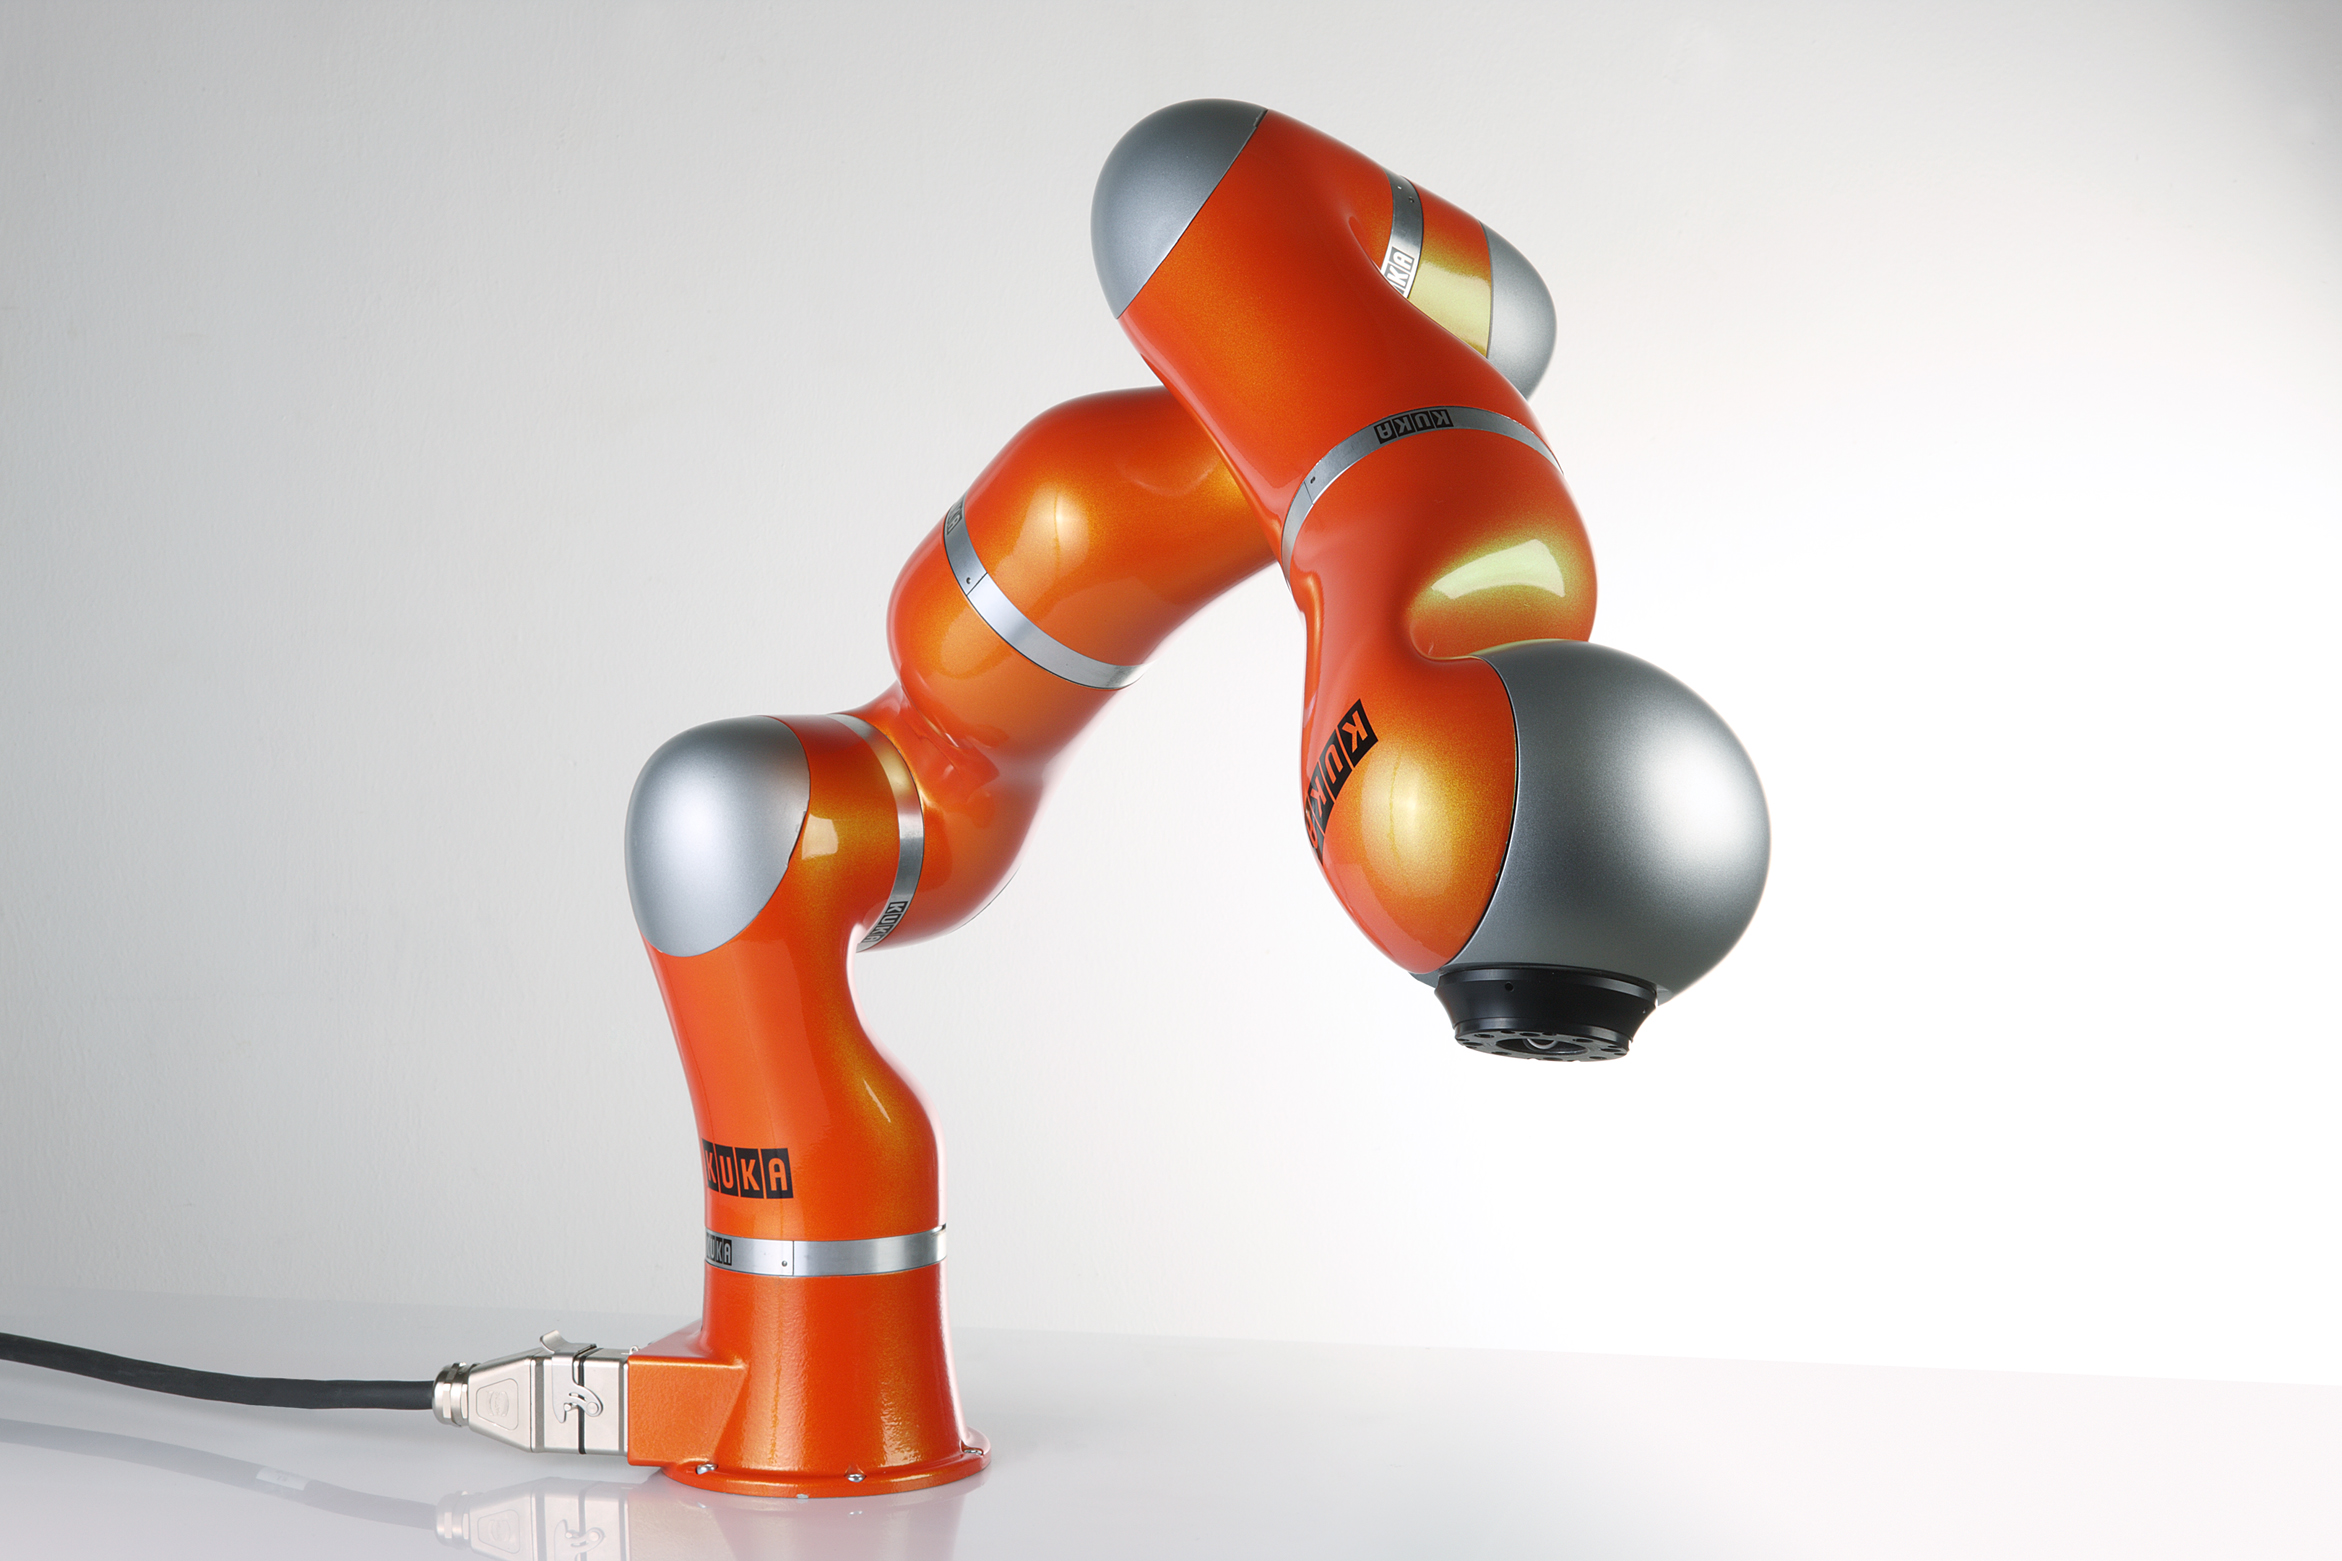
\includegraphics[scale=0.5]{KUKA.jpg}
  \caption{KUKA LWR$4+$ manipulator. \label{fig:kuka_lwr}}
\end{figure}
\par
In order to send the control laws, described in the previous sections, to the robot
 one of the internal modes of operation, called Joints Specific Impedance, was used
\[
\boldsymbol{\tau}_{cmd} = K_j(\vec{q}_{FRI} - \vec{q}_{msr}) + D(d_{j}) + \boldsymbol{\tau}_{FRI} + \vec{f}_{dynamics}(\vec{q}, \dot{\vec{q}}, \ddot{\vec{q}})
\]
where $\boldsymbol{\tau}_{cmd}$ is the effective torque sent to the robot, 
$\vec{q}_{FRI}$ is the vector of the desired angular positions of the joints, 
$\vec{q}_{msr}$ is the vector of the angular positions of the joints, 
$K_j$ and $D(d_j)$ are gains that shape the dynamics of the impedance control mode,
$\boldsymbol{\tau}_{FRI}$ is an additional torque provided by the user and 
$\vec{f}_{dynamics}(\vec{q}, \dot{\vec{q}}, \ddot{\vec{q}})$ is a gravity compensation
term provided by the producer.
\par
Since the control laws developed are pure torque laws only the term
$\boldsymbol{\tau}_{FRI}$ was used and the others were set as:
\begin{itemize}
\item[-] $K_j = 0$;
\item[-] $d_j = 0$;
\item[-] $\vec{q}_{FRI} = \vec{q}_{msr}$
\end{itemize}

\subsubsection{Force Torque sensor}
The force/torque sensor used in this work is an ATI Mini$45$ (cite).
In all the experiments the measured signal was filtered using a built-in
LP filter with cutoff frequency of $\SI{8}{Hz}$.

\subsubsection{Notes about controllers implementation}
In order to implement the control laws
\[
\begin{split}
  \vec{\tau} &= \\
  \vec{\tau} &= C \dot{\vec{q}} + {}^{b}J^{T}_{F} ( B_A \vec{a} - B_A {}^{ws} \dot{J_{A,E}} \dot{\vec{q}} + {}^b\vec{w}_{F}) +
  (I_7 - ({}^{b}J^{T}_{F}) ({}^{b} \bar{J}^{T}_{F})) \vec{\gamma}_{0}
\end{split}
\]
several quantities are required among which
\begin{itemize}
\item[-] angular position, velocity and acceleration of the joints;
\item[-] Jacobians;
\item[-] inertia matrix;
\item[-] Coriolis matrix;
\item[-] direct and inverse kinematics facilities;
\item[-] Euler ZYZ kinematical matrix.
\end{itemize}
\par
The angular position are provided by the FRI software layer.
The angular velocities and the angular accelerations are not provided by
the producer so they were estimated using an exponential smoothing filter of the 
form
\[
\begin{cases}
  \dot{\vec{q}}_0 = \vec{0} \\
  \dot{\vec{q}}_k = (1 - \alpha) \dot{\vec{q}}_{k-1} + \alpha \frac{\vec{q}_k - \vec{q}_{k-1}}{t_s}
\end{cases}
\]
\[
\begin{cases}
  \ddot{\vec{q}}_0 = \vec{0} \\
  \ddot{\vec{q}}_k = (1 - \alpha) \ddot{\vec{q}}_{k-1} + \alpha \frac{\dot{\vec{q}}_k - \dot{\vec{q}}_{k-1}}{t_s}
\end{cases}
\]
where the constant $\alpha \in [0, 1]$ is the smoothing factor and $t_s$ is the sampling time.
In all the experiments $\alpha = 0.2$ and $t_s = \SI{3}{ms}$.
\par
All the others quantities were evaluated numerically using the facilities offered by the KDL library which was
integrated into the already existing KUKA LWR$4+$ software stack provided to the students

\subsection{Experiment 1}
In this experiment (fig. \ref{fig:hand_button}) the robot is supposed to press an emergency button.
\begin{figure}[h]
  \centering
  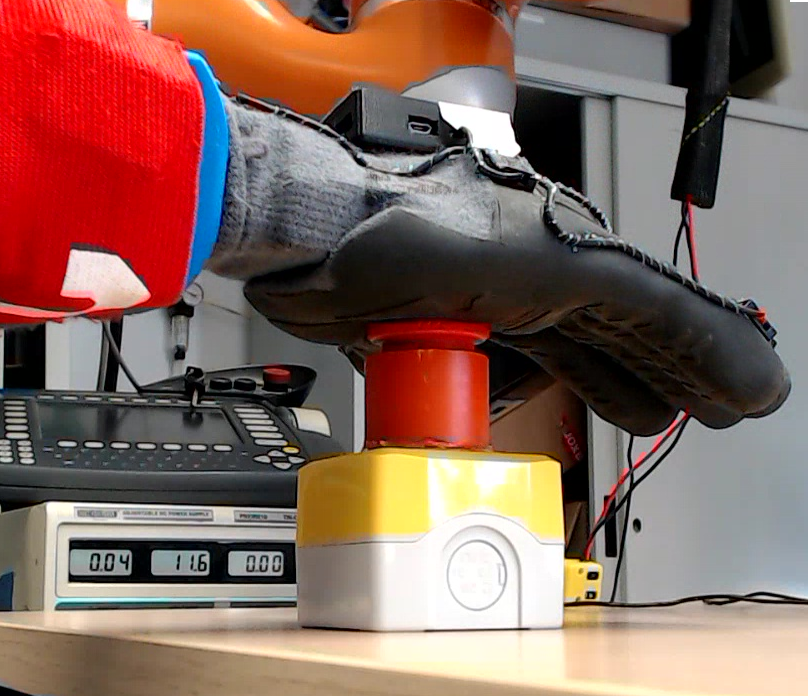
\includegraphics[scale=0.37]{hand_button.png}
  \caption{The hand while it presses the emergency button. \label{fig:hand_button}}
\end{figure}
\par
Initially a reference command of approximately $\SI{1}{N}$ is sent to the robot
until the contact takes place. Then several set points are sent to the robot:
\begin{itemize}
\item[-] $F_{z,des} = \SI{-2.5}{N}$
\item[-] $F_{z,des} =\SI{-1.5}{N}$
\item[-] $F_{z,des} =\SI{-3.5}{N}$
\item[-] $F_{z,des} =\SI{-1}{N}$
\end{itemize}
\par
The results, presented in the Table \ref{fig:button},
\begin{table}[h]
  \begin{tabular}{cc}
    \begin{subfigure}{0.5\textwidth}
      \centering
      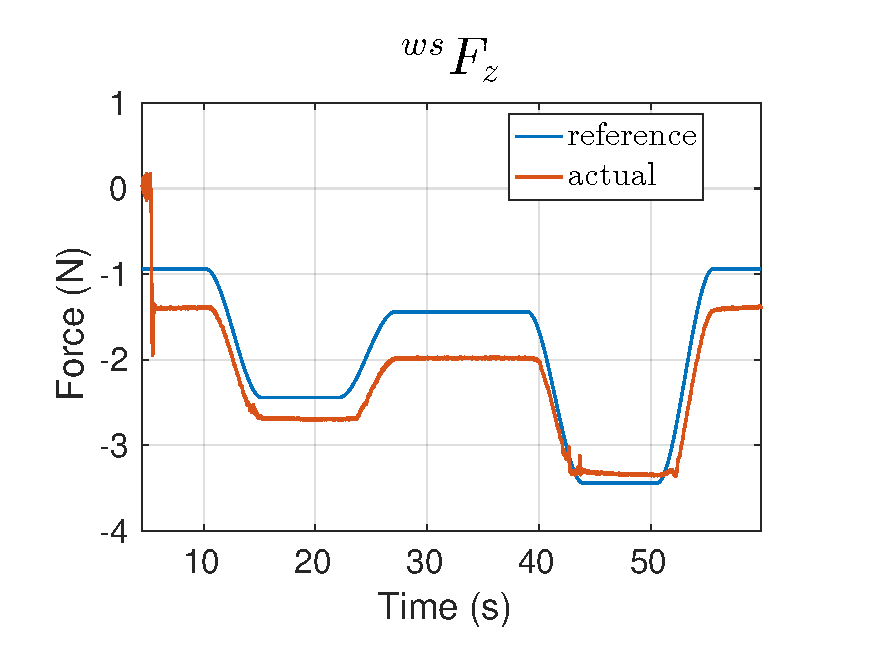
\includegraphics[scale=0.5]{button_z}
      \caption{Reference and actual force. \label{fig:button_z}}
    \end{subfigure}&
    \begin{subfigure}{0.5\textwidth}
      \centering
      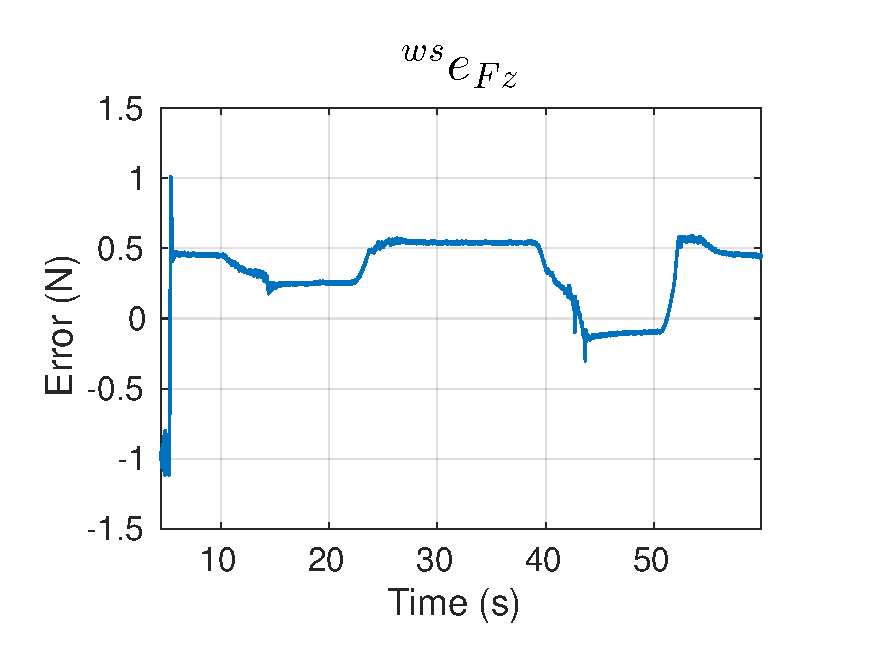
\includegraphics[scale=0.5]{button_err_z}
      \caption{Error. \label{fig:button_error_z}}
    \end{subfigure} 
  \end{tabular}
  \caption{Experiment 1, the hand presses a button.\\
  $K_f = 2$ and $B_f = 45$\label{fig:button}}
\end{table}
show that the error after the contact phase is bounded between
$\SI{-0.35}{N}$ and $\SI{0.5}{N}$ and it decreases as the requested force 
increases. The contact phase is visible as a spike in the measured force
(see Table \ref{fig:button_z}).

\subsection{Experiment 2}
In this experiment (Fig. \ref{fig:hand_banana}) a banana is dragged 
on a table while the contact force between the hand and the fruit is regulated.
\begin{figure}[h]
  \centering
  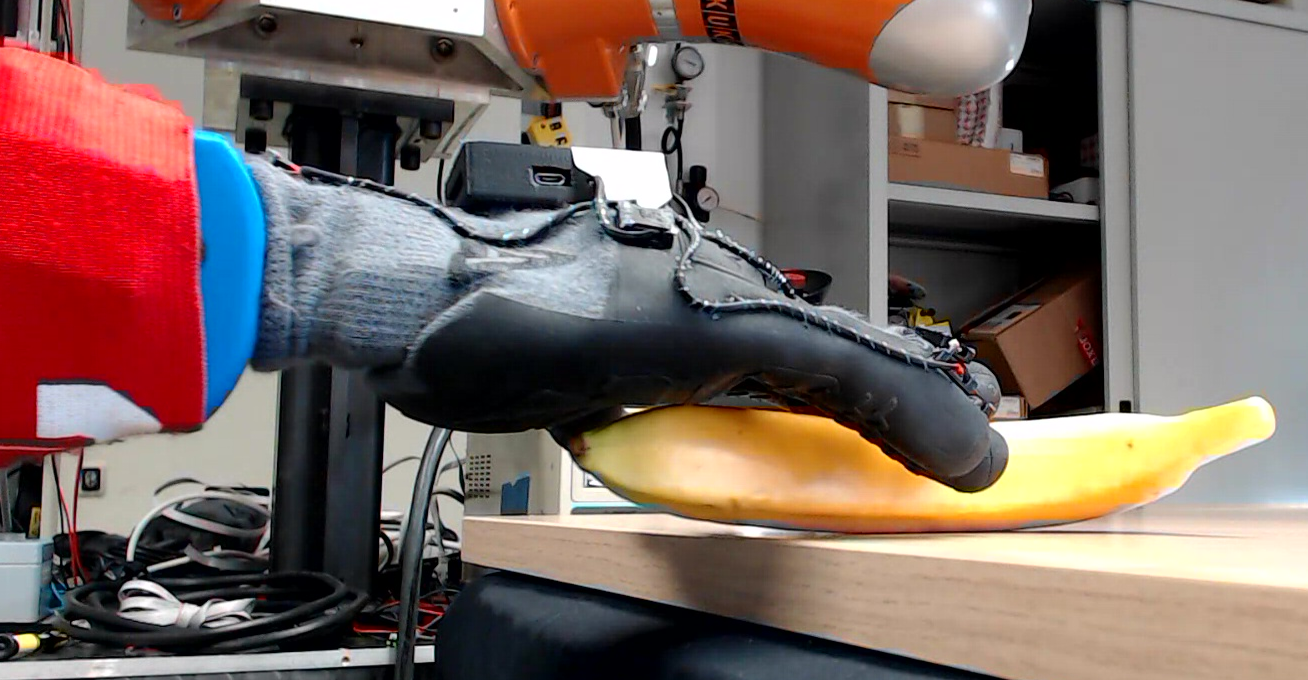
\includegraphics[scale=0.25]{hand_banana.png}
  \caption{The hand while it drags the banana. \label{fig:hand_banana}}
\end{figure}
The object is dragged in $\SI{5}{s}$ for a distance of $\SI{12}{cm}$ and the requested force is $\SI{3}{N}$.
In the Table \ref{fig:banana} only the results of the dragging phase are shown.
\begin{table}[h]
  \begin{tabular}{cc}
    \begin{subfigure}{0.5\textwidth}
      \centering
      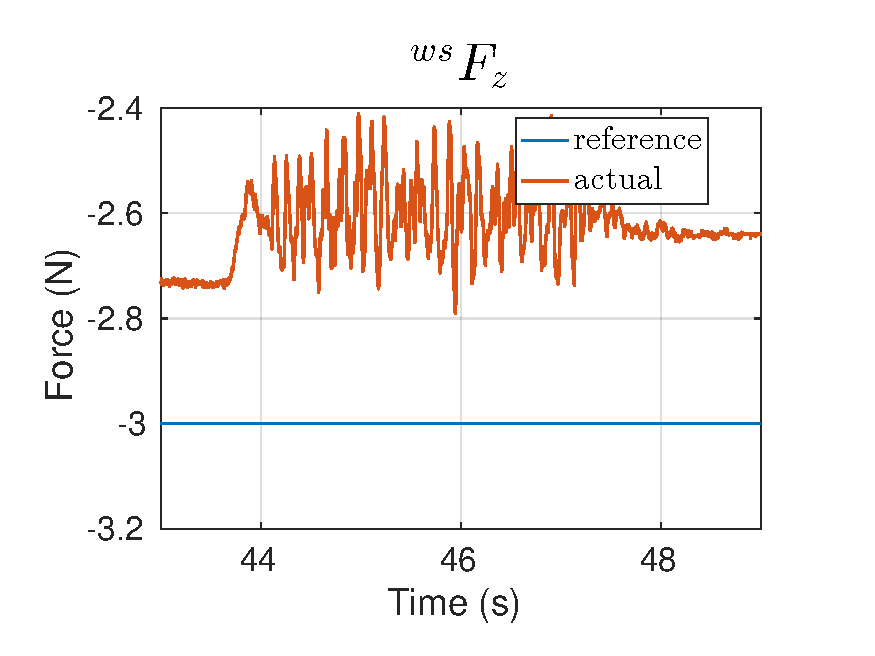
\includegraphics[scale=0.5]{banana_z}
      \caption{Reference and actual force. \label{fig:banana_z}}
    \end{subfigure}&
    \begin{subfigure}{0.5\textwidth}
      \centering
      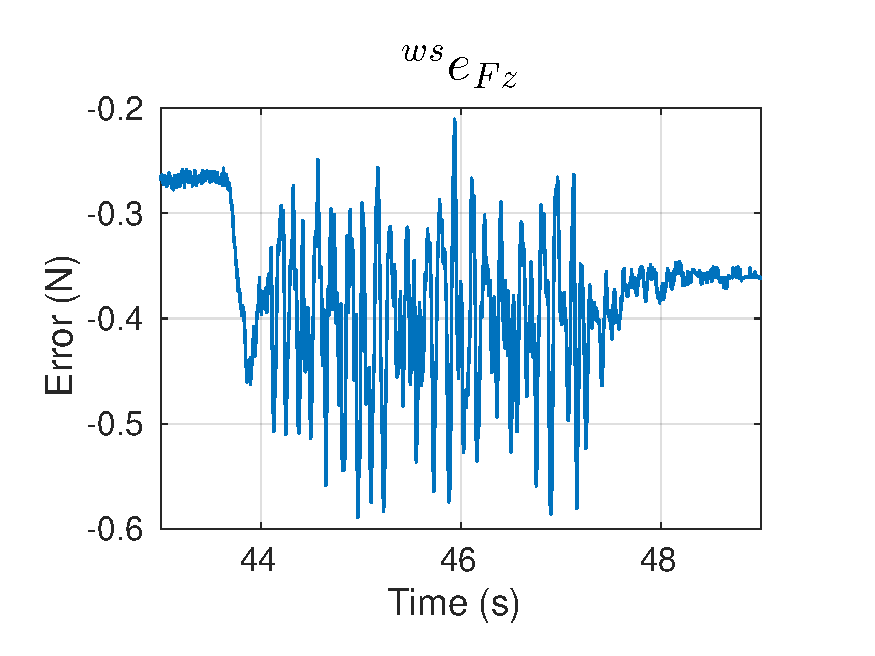
\includegraphics[scale=0.5]{banana_err_z}
      \caption{Error. \label{fig:banana_error_z}}
    \end{subfigure}\\
    \begin{subfigure}{0.5\textwidth}
      \centering
      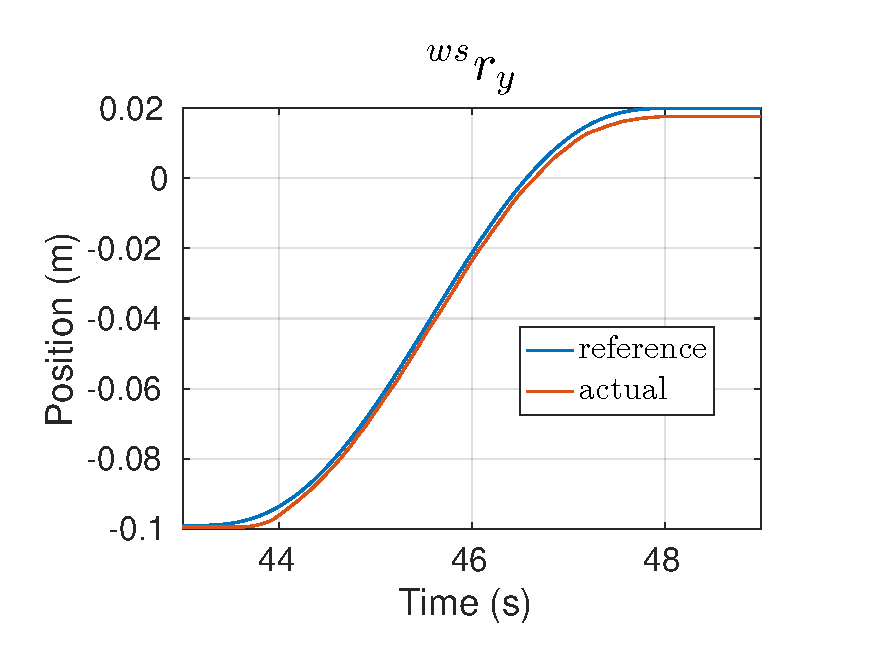
\includegraphics[scale=0.5]{banana_y}
      \caption{Reference and actual trajectory. \label{fig:banana_y}}
    \end{subfigure}&
    \begin{subfigure}{0.5\textwidth}
      \centering
      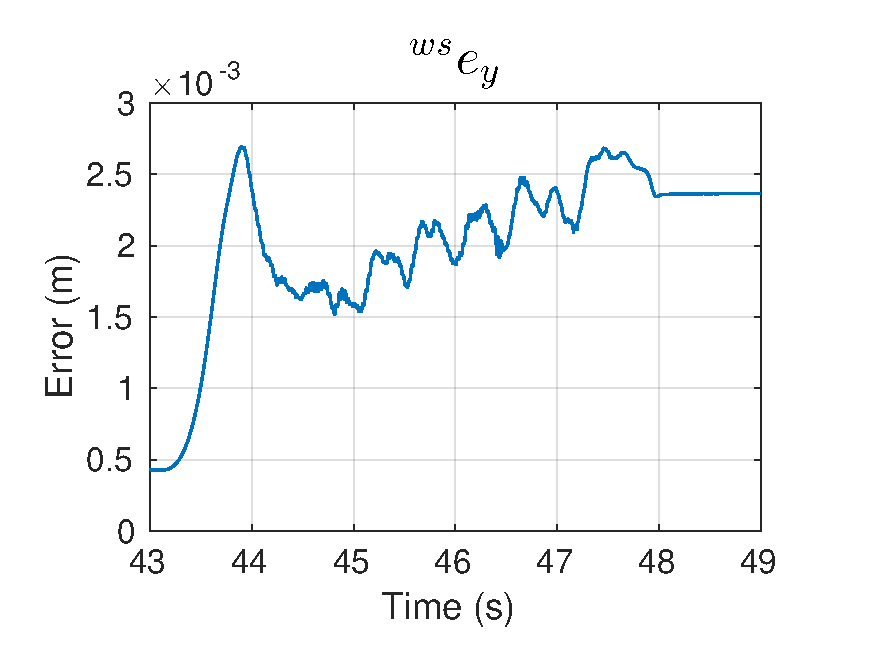
\includegraphics[scale=0.5]{banana_err_y}
      \caption{Error. \label{fig:banana_error_y}}
    \end{subfigure}
  \end{tabular}
  \caption{Experiment 2, the hand drags a banana.\\
  $K_f = 2.5$ and $B_f = 85$.}\label{fig:banana}
\end{table}
Although the force error is bounded between $\SI{-0.6}{N}$ and 
$\SI{-0.25}{N}$ undesired spikes are present because of
the vibrations due to the movement.

\subsection{Experiment 3}
\newpage

\newpage
%% \nocite{*}
\bibliography{bibliography}
\bibliographystyle{ieeetr}
\end{document}
